\documentclass[a4paper,11pt]{article}
\usepackage{zh_CN-Adobefonts_external} % Simplified Chinese Support using external fonts (./fonts/zh_CN-Adobe/)
\usepackage{fancyhdr}  % 页眉页脚
\usepackage{minted}    % 代码高亮
\usepackage[colorlinks]{hyperref}  % 目录可跳转
\setlength{\headheight}{15pt}
\usepackage[left=1.5cm,right=1.5cm,top=1.5cm,bottom=1.5cm]{geometry}

% 定义页眉页脚
\pagestyle{fancy}
\fancyhf{}
\fancyhead[C]{Algorithm Library by palayutm}
\lfoot{}
\cfoot{\thepage}
\rfoot{}

\author{palayutm}   
\title{Algorithm Library}

\begin{document} 
	\maketitle % 封面
	\newpage % 换页
	\newpage
	\tableofcontents % 目录
	\newpage
	\section{计算几何}
%\cleardoublepage
\subsection{二维基础}
\inputminted[breaklines]{cpp}{./computational_geometry/two_dimensions_basic.cpp}
\subsection{三角形公式}
	\subsubsection{三角形内心}
	$\frac{a \vec{A} + b \vec{B} + c \vec{C}}{a + b + c}$
	\subsubsection{三角形外心}
	$\frac{\vec{A} + \vec{B} - \frac{\vec{BC} \cdot \vec{CA}}{\vec{AB} \times \vec{BC}} \vec{AB}^T}{2}$
	\subsubsection{三角形垂心}
	$\vec{H} = 3 \vec{G} - 2 \vec{O}$
	\subsubsection{三角形旁心}
	$\frac{-a \vec{A} + b \vec{B} + c \vec{C}}{-a + b + c}$ (其余两点同理)
	\subsubsection{三角形外接圆半径}
	$R = \frac{abc}{4S}$
	\subsubsection{海伦公式}
	$$
	2s = a + b + c \\
	S = \sqrt{s(s - a)(s - b)(s - c)}
	$$
	\subsubsection{皮克公式}
	顶点全都在格子上的简单多边形的面积$S$可由边上的格点数$B$、内部的格点数$I$表示为 \\
	$S = \frac{B}{2} + I - 1$
\subsection{半平面交}
\inputminted[breaklines]{cpp}{./computational_geometry/half_plane_intersection.cpp}
\subsection{二维最小圆覆盖}
\inputminted[breaklines]{cpp}{./computational_geometry/2D-minimum-circle-coverage.cpp}
\subsection{凸包}
\inputminted[breaklines]{cpp}{./computational_geometry/convex_hull.cpp}
\subsection{凸包游戏}
\inputminted[breaklines]{cpp}{./computational_geometry/convex_hull_game.cpp}
\subsection{圆并}
\inputminted[breaklines]{cpp}{./computational_geometry/circle_union.cpp}
\subsection{最远点对}
\inputminted[breaklines]{cpp}{./computational_geometry/farthest_point_pair.cpp}
\subsection{根轴}
���ᶨ�壺����ԲԲ����ȵĵ��γɵ�ֱ��

��Բ$\{(x_1, y_1), r_1\}$��$\{(x_2, y_2), r_2\}$�ĸ��᷽�̣�

$2(x_2 - x_1)x + 2(y_2 - y_1)y + f_1 - f_2 = 0$������$f_1 = {x_1} ^ 2 + {y_1} ^ 2 - {r_1} ^ 2, f_2 = {x_2} ^ 2 + {y_2} ^ 2 - {r_2} ^ 2$��

\subsection{Farmland - 平面图转对偶图}
\inputminted[breaklines]{cpp}{./computational_geometry/Farmland.cpp}
\subsection{三维基础}
	\inputminted[breaklines]{cpp}{./computational_geometry/three_dimensions_basic.cpp}
	两点在平面同侧:与法向量的点积符号相同 \\
	两直线平行/垂直:同二维 \\
	平面平行/垂直:判断法向量 \\
	线面垂直:法向量和直线平行 \\
	判断空间线段是否相交:四点共面两线段不平行相互在异侧 \\
	线段和三角形是否相交:线段在三角形平面不同侧三角形任意两点在线段和第三点组成的平面的不同侧 \\
	求平面交线:取一平面与另一平面不平行的一条直线与另一平面的交点,以及法向量叉积得到直线方向 \\
	点到直线距离:叉积得到三角形的面积除以底边 \\
	点到平面距离:点积法向量 \\
	直线间距离:平行时随便取一点求距离,否则叉积方向向量得到方向点积计算长度 \\
	直线夹角:点积  平面夹角:法向量点积
\subsection{三维凸包}
\inputminted[breaklines]{cpp}{./computational_geometry/convex_hull_3dim.cpp}
	\twocolumn
	\section{字符串}
%\cleardoublepage
\subsection{manacher}
\inputminted[breaklines]{cpp}{./string/manacher.cpp}
\subsection{后缀数组}
\inputminted[breaklines]{cpp}{./string/SA.cpp}
\subsection{后缀自动机}
\inputminted[breaklines]{cpp}{./string/SAM.cpp}
\subsection{广义后缀自动机}
\inputminted[breaklines]{cpp}{./string/general_SAM.cpp}
\subsection{回文自动机}
\inputminted[breaklines]{cpp}{./string/pam.cpp}
\subsection{Lyndon Word Decomposition  NewMeta}
\inputminted[breaklines]{cpp}{./string/Lyndon_Word_Decomposition-NewMeta.cpp}
\subsection{EXKMP  NewMeta}
\inputminted[breaklines]{cpp}{./string/EXKMP-NewMeta.cpp}
	%\section{数据结构}
%\cleardoublepage
\subsection{Link-Cut-Tree}
\inputminted[breaklines]{cpp}{./data-structure/LinkCutTree.cpp}
\subsection{KDTree}
\inputminted[breaklines]{cpp}{./data-structure/KDTree.cpp}
\subsection{莫队上树}
Let dfn_s[u] <= dfn_s[v]. 
If u is v's ancient, query(dfn_s[u], dfn_s[v]). 
Else query(dfn_t[u], dfn_s[v]) + lca(u, v). 

	%\section{图论}
%\cleardoublepage
\subsection{点双连通分量}
\inputminted[breaklines]{cpp}{./graph-theory/vertex-biconnected-component.cpp}
\subsection{边双连通分量}
\inputminted[breaklines]{cpp}{./graph-theory/edge-biconnected-component.cpp}
\subsection{有根树同构-Reshiram}
\inputminted[breaklines]{cpp}{./graph-theory/rooted-tree-isomorphism-Reshiram.cpp}
\subsection{Hopcraft-Karp}
\inputminted[breaklines]{cpp}{./graph-theory/Hopcroft-Karp.cpp}
\subsection{ISAP}
\inputminted[breaklines]{cpp}{./graph-theory/ISAP-maximum-flow.cpp}
\subsection{zkw费用流}
\inputminted[breaklines]{cpp}{./graph-theory/zkw-cost-flow.cpp}
\subsection{无向图全局最小割}
\inputminted[breaklines]{cpp}{./graph-theory/StoerWagner.cpp}
\subsection{KM}
\inputminted[breaklines]{cpp}{./graph-theory/KM-Algorithm.cpp}
\subsection{一般图最大权匹配}
\inputminted[breaklines]{cpp}{./graph-theory/general-graph-maximum-weight-matching.cpp}
\subsection{最大团搜索}
\inputminted[breaklines]{cpp}{./graph-theory/maximum-clique.cpp}
\subsection{极大团计数}
\inputminted[breaklines]{cpp}{./graph-theory/maximum-clique-counting.cpp}
\subsection{虚树-NewMeta}
\inputminted[breaklines]{cpp}{./graph-theory/virtual-tree-NewMeta.cpp}
\subsection{2-Sat}
\inputminted[breaklines]{cpp}{./graph-theory/2-sat.cpp}
\subsection{支配树}
\inputminted[breaklines]{cpp}{./graph-theory/dominator-tree.cpp}

\subsection{哈密顿回路}
\inputminted[breaklines]{cpp}{./graph-theory/hamilton-loop.tex}
\subsection{曼哈顿最小生成树}
\inputminted[breaklines]{cpp}{./graph-theory/manhattan-minimum-spanning-tree.tex}

\subsection{弦图}
\begin{enumerate}
\item[1.] 团数 $\leq$ 色数 , 弦图团数 = 色数

\item[2.] 设 $next(v)$ 表示 $N(v)$ 中最前的点 . 
令 w* 表示所有满足 $A \in B$ 的 w 中最后的一个点 , 
判断 $v \cup N(v)$ 是否为极大团 , 
只需判断是否存在一个 w, 
满足 $Next(w)=v$ 且 $|N(v)| + 1 \leq |N(w)|$ 即可 . 

\item[3.] 最小染色 : 完美消除序列从后往前依次给每个点染色 , 
给每个点染上可以染的最小的颜色

\item[4.] 最大独立集 : 完美消除序列从前往后能选就选

\item[5.] 弦图最大独立集数 $=$ 最小团覆盖数 , 
最小团覆盖 : 
设最大独立集为 $\{p_1,p_2, \dots ,p_t\}$, 
则 $\{p_1\cup N(p_1), \dots , p_t \cup N(p_t)\}$ 
为最小团覆盖
\end{enumerate}

\subsection{图同构 hash}

$$F_t(i) = 
    (F_{t-1}(i) \times A + 
    \sum_{i\rightarrow j} F_{t-1}(j) \times B + 
    \sum_{j\rightarrow i} F_{t-1}(j) \times C +
    D \times (i = a))\ mod\ P
$$

枚举点 a , 迭代 K 次后求得的就是 a 点所对应的 hash 值 

其中 K , A , B , C , D , P 为 hash 参数 , 可自选

	%\section{字符串}
%\cleardoublepage
\subsection{manacher}
\inputminted[breaklines]{cpp}{./string/manacher.cpp}
\subsection{后缀数组}
\inputminted[breaklines]{cpp}{./string/SA.cpp}
\subsection{后缀自动机}
\inputminted[breaklines]{cpp}{./string/SAM.cpp}
\subsection{广义后缀自动机}
\inputminted[breaklines]{cpp}{./string/general_SAM.cpp}
\subsection{回文自动机}
\inputminted[breaklines]{cpp}{./string/pam.cpp}
\subsection{Lyndon Word Decomposition  NewMeta}
\inputminted[breaklines]{cpp}{./string/Lyndon_Word_Decomposition-NewMeta.cpp}
\subsection{EXKMP  NewMeta}
\inputminted[breaklines]{cpp}{./string/EXKMP-NewMeta.cpp}
	%\section{数学}
\subsection{prime}
\subsubsection{miller-rabin}
\inputminted[breaklines]{cpp}{math/prime/miller-rabin.cpp}
\subsubsection{pollard-rho}
\inputminted[breaklines]{cpp}{math/prime/pollard-rho.cpp}
\subsubsection{求原根}
\inputminted[breaklines]{cpp}{math/prime/get-primitive-root.cpp}
\subsection{多项式}
\subsubsection{快速傅里叶变换}
\inputminted[breaklines]{cpp}{math/polynomial/FFT.cpp}
\subsubsection{快速数论变换}
\inputminted[breaklines]{cpp}{math/polynomial/NTT.cpp}
	%\section{杂项}
%\cleardoublepage
\subsection{fread 读入优化}
\inputminted[breaklines]{cpp}{./hint/input-acceleration.cpp}
\subsection{真正释放STL内存}
\inputminted[breaklines]{cpp}{./hint/STL-memory-release.cpp}
\subsection{梅森旋转算法}
\inputminted[breaklines]{cpp}{./hint/mersenne-twister.cpp}
\subsection{蔡勒公式}
\inputminted[breaklines]{cpp}{./hint/zeller.cpp}
\subsection{开栈}
\inputminted[breaklines]{cpp}{./hint/openstack.cpp}
\subsection{Size为k的子集}
\inputminted[breaklines]{cpp}{./hint/subset-of-size-k.cpp}
\subsection{长方体表面两点最短距离}
\inputminted[breaklines]{cpp}{./hint/distance-on-surface-of-cuboid.cpp}
\subsection{32-bit/64-bit随机素数}
\begin{tabular}{|l|l|}
	\hline
	\texttt{32-bit} & \texttt{64-bit} \\
	\hline
	73550053 & 1249292846855685773 \\
	\hline
	148898719 & 1701750434419805569 \\
	\hline
	189560747 & 3605499878424114901 \\
	\hline
	459874703 & 5648316673387803781 \\
	\hline
	1202316001 & 6125342570814357977 \\
	\hline
	1431183547 & 6215155308775851301 \\
	\hline
	1438011109 & 6294606778040623451 \\
	\hline
	1538762023 & 6347330550446020547 \\
	\hline
	1557944263 & 7429632924303725207 \\
	\hline
	1981315913 & 8524720079480389849 \\
	\hline
\end{tabular}

\subsection{NTT 素数及其原根}
\begin{tabular}{|l|l|}
	\hline
	\texttt{Prime} & \texttt{Primitive root} \\
	\hline
	1053818881 & 7 \\
	\hline
	1051721729 & 6 \\
	\hline
	1045430273 & 3 \\
	\hline
	1012924417 & 5 \\
	\hline
	1007681537 & 3 \\
	\hline
	1000000000622593 & 5 \\
	\hline
\end{tabular}

\subsection{伯努利数-Reshiram}
\begin{enumerate}
	\item 初始化:$B_0(n) = 1$
	\item 递推公式:
	\[B_m(n) = n^m - \sum_{k = 0}^{m - 1}\binom{m}{k} \frac{B_k(n)}{m - k + 1}\]
	\item 应用:
	\[\sum_{k = 1}^{n} k^m = \frac{1}{m + 1}\sum_{k = 0}^{m}\binom{m + 1}{k}n^{m + 1 - k}\]
\end{enumerate}



\subsection{博弈游戏-Reshiram}
\subsubsection{巴什博奕}
	\begin{enumerate}
		\item 
			只有一堆n个物品,两个人轮流从这堆物品中取物,规定每次至少取一个,最多取m个。最后取光者得胜。
		\item
			显然,如果$n=m+1$,那么由于一次最多只能取$m$个,所以,无论先取者拿走多少个,
			后取者都能够一次拿走剩余的物品,后者取胜。因此我们发现了如何取胜的法则:如果
			$n=(m+1)r+s$,(r为任意自然数,$s \leq m$),那么先取者要拿走$s$个物品,
			如果后取者拿走$k(k \leq m)$个,那么先取者再拿走$m+1-k$个,结果剩下$(m+1)(r-1)$
			个,以后保持这样的取法,那么先取者肯定获胜。总之,要保持给对手留下$(m+1)$的倍数,
			就能最后获胜。
	\end{enumerate}
\subsubsection{威佐夫博弈}
	\begin{enumerate}
		\item 
			有两堆各若干个物品,两个人轮流从某一堆或同时从两堆中取同样多的物品,规定每次至少取
			一个,多者不限,最后取光者得胜。
		\item
			判断一个局势$(a, b)$为奇异局势(必败态)的方法:
			$$a_k =[k (1+\sqrt{5})/2],b_k= a_k + k$$
	\end{enumerate}
\subsubsection{阶梯博奕}
	\begin{enumerate}
		\item
			博弈在一列阶梯上进行,每个阶梯上放着自然数个点,两个人进行阶梯博弈,
			每一步则是将一个阶梯上的若干个点(至少一个)移到前面去,最后没有点
			可以移动的人输。
		\item
			解决方法:把所有奇数阶梯看成N堆石子,做NIM。(把石子从奇数堆移动到偶数
			堆可以理解为拿走石子,就相当于几个奇数堆的石子在做Nim)
	\end{enumerate}
\subsubsection{图上删边游戏}
	\subsubsection{链的删边游戏}
		\begin{enumerate}
			\item
				游戏规则:对于一条链,其中一个端点是根,两人轮流删边,脱离根的部分也算被删去,最后没边可删的人输。
			\item
				做法:$sg[i] = n - dist(i) - 1$(其中$n$表示总点数,$dist(i)$表示离根的距离)
		\end{enumerate}
	\subsubsection{树的删边游戏}
		\begin{enumerate}
			\item
				游戏规则:对于一棵有根树,两人轮流删边,脱离根的部分也算被删去,没边可删的人输。
			\item
				做法:叶子结点的$sg=0$,其他节点的$sg$等于儿子结点的$sg+1$的异或和。
		\end{enumerate}
	\subsubsection{局部连通图的删边游戏}
		\begin{enumerate}
			\item
				游戏规则:在一个局部连通图上,两人轮流删边,脱离根的部分也算被删去,没边可删的人输。
				局部连通图的构图规则是,在一棵基础树上加边得到,所有形成的环保证不共用边,且只与基础树有一个公共点。
			\item
				做法:去掉所有的偶环,将所有的奇环变为长度为1的链,然后做树的删边游戏。
		\end{enumerate}


\subsection{Formulas}
\def \bangle{ \atopwithdelims \langle \rangle}
\begin{small}
\subsubsection{Arithmetic Function}
\[ \sigma_k(n) = \sum_{d|n}d^k = \prod_{i=1}^{\omega(n)}\frac{p_i^{(a_i+1)k}-1}
{p_i^k-1} \]
\[ J_k(n) = n^k\prod_{p|n}(1-\frac{1}{p^k}) \]
$J_k(n)$ is the number of $k$-tuples of positive integers all less than or equal to n that form a coprime $(k + 1)$-tuple together with $n$.
\[ \sum_{\delta|n}J_k(\delta) = n^k \]
\[ \sum_{\delta|n}\delta^sJ_r(\delta)J_s(\frac{n}{\delta}) = J_{r+s}(n) \]
\begin{align*}
\sum_{\delta|n}\varphi(\delta)d(\frac{n}{\delta}) = \sigma(n),&\ \sum_{\delta|n}\left| \mu(\delta) \right| = 2^{\omega(n)} \\
\sum_{\delta|n}2^{\omega(\delta)} = d(n^2),&\ \sum_{\delta|n}d(\delta^2) = d^2(n) \\
\sum_{\delta|n}d(\frac{n}{\delta})2^{\omega(\delta)} = d^2(n),&\ \sum_{\delta|n}\frac{\mu(\delta)}{\delta} = \frac{\varphi(n)}{n} \\
\sum_{\delta|n}\frac{\mu(\delta)}{\varphi(\delta)} = d(n),&\ \sum_{\delta|n}\frac{\mu^2(\delta)}{\varphi(\delta)} = \frac{n}{\varphi(n)} \\
\end{align*}
\[ n|\varphi(a^n-1) \]
\[ \sum_{\substack{1 \leq k \leq n \\ \gcd(k, n) = 1}}f(\gcd(k-1, n)) = \varphi(n)
\sum_{d|n}\frac{(\mu*f)(d)}{\varphi(d)} \]
\[ \varphi(\mathrm{lcm}(m, n))\varphi(\gcd(m,n)) = \varphi(m)\varphi(n) \]
\[ \sum_{\delta|n}d^3(\delta) = (\sum_{\delta|n}d(\delta))^2 \]
\[ d(uv) = \sum_{\delta|\gcd(u, v)}\mu(\delta)d(\frac{u}{\delta})d(\frac{v}{\delta}) \]
\[ \sigma_k(u)\sigma_k(v) = \sum_{\delta|\gcd(u, v)}\delta^k\sigma_k(\frac{uv}{\delta^2}) \]
\[ \mu(n) = \sum_{k=1}^n[\gcd(k, n)=1]\cos{2\pi \frac{k}{n}} \]
\[ \varphi(n) = \sum_{k=1}^n[\gcd(k, n)=1] = \sum_{k=1}^n\gcd(k, n)\cos{2\pi \frac{k}{n}} \]
\[
\left\{
\begin{aligned}
&S(n) = \sum_{k=1}^n(f \ast g)(k) \\
&\sum_{k=1}^nS(\lfloor {n \over k} \rfloor) = \sum_{i=1}^nf(i)\sum_{j=1}^{\lfloor{n \over i}\rfloor}(g \ast 1)(j)
\end{aligned}
\right.
\]
\[
\left\{
\begin{aligned}
&S(n) = \sum_{k=1}^n(f \cdot g)(k), g \text{ completely multiplicative} \\
&\sum_{k=1}^nS(\lfloor {n \over k} \rfloor)g(k) = \sum_{k=1}^n(f \ast 1)(k)g(k)
\end{aligned}
\right.
\]
\subsubsection{Binomial Coefficients}
\[ {n \choose k} = (-1)^k{k-n-1 \choose k} \]
\[ \sum_{k \leq n}{r+k \choose k} = {r+n+1 \choose n} \]
\[ \sum_{k=0}^n{k \choose m} = {n+1 \choose m+1} \]
\[ \sqrt{1+z} = 1 + \sum_{k=1}^{\infty}\frac{(-1)^{k-1}}{k\times2^{2k-1}}{2k-2 \choose k-1}z^k \]
\[ \sum_{k=0}^{r}{r-k \choose m}{s+k \choose n} = {r+s+1 \choose m+n+1} \]
\[ C_{n, m} = {n+m \choose m} - {n+m \choose m-1}, n \geq m \]
\[ {n \choose k} \equiv [n\& k=k] \pmod 2 \]
\subsubsection{Fibonacci Numbers}
\[ F(z) = \frac{z}{1-z-z^2} \]
\[ f_n = \frac{{\phi}^n-{\hat{\phi}}^n}{\sqrt{5}}, \phi = \frac{1+\sqrt{5}}{2},
\hat{\phi} = \frac{1-\sqrt{5}}{2} \]
\[ \sum_{k=1}^nf_k = f_{n+2}-1 \]
\[ \sum_{k=1}^nf^2_k = f_nf_{n+1} \]
\[ \sum_{k=0}^nf_kf_{n-k} = \frac{1}{5}(n-1)f_n+\frac{2}{5}nf_{n-1} \]
\[ f^2_n + (-1)^n = f_{n+1}f_{n-1} \]
\[ f_{n+k} = f_nf_{k+1} + f_{n-1}f_k \]
\[ f_{2n+1} = f^2_n+f^2_{n+1} \]
\[ (-1)^kf_{n-k} = f_{n}f_{k-1} - f_{n-1}f_{k} \]
\[ \text{Modulo }f_n, f_{mn+r} \equiv \left\{
\begin{aligned}
&f_r,& m \bmod 4 = 0; \\
&(-1)^{r+1}f_{n-r},& m \bmod 4 = 1; \\
&(-1)^nf_r,& m \bmod 4 = 2; \\
&(-1)^{r+1+n}f_{n-r},& m \bmod 4 = 3.
\end{aligned}
\right.
\]
\subsubsection{Stirling Cycle Numbers}
\begin{align*}
 {n+1 \brack k} = n{n \brack k} + {n \brack k-1},&\ \  {n+1 \brack 2} = n!H_n \\
x^{\underline{n}} = \sum_k{ {n \brack k}(-1)^{n-k}x^k },&\ \  x^{\overline{n}} = \sum_k{ {n \brack k}x^k } \\
 \end{align*}
\subsubsection{Stirling Subset Numbers}
\[ {n+1 \brace k} = k{n \brace k} + {n \brace k-1} \]
\[ x^n = \sum_k{ {n \brace k}x^{\underline{k}} } = \sum_k{ {n \brace k}(-1)^{n-k}x^{\overline{k}} } \]
\[ m!{n \brace m} = \sum_k{m \choose k}k^n(-1)^{m-k} \]
\subsubsection{Eulerian Numbers}
\[ {n \bangle k} = (k+1){n-1 \bangle k} + (n-k){n-1 \bangle k-1} \]
\[ x^n = \sum_k{ {n \bangle k}{x+k \choose n} } \]
\[ {n \bangle m} = \sum_{k=0}^m{n+1 \choose k}(m+1-k)^n(-1)^k \]
\subsubsection{Harmonic Numbers}
\[ \sum_{k=1}^nH_k = (n+1)H_n-n \]
\[ \sum_{k=1}^nkH_k = \frac{n(n+1)}{2}H_n - \frac{n(n-1)}{4} \]
\[ \sum_{k=1}^n{k \choose m}H_k = {n+1 \choose m+1}(H_{n+1} - \frac{1}{m+1}) \]
\subsubsection{Pentagonal Number Theorem}
\[ \prod_{n=1}^{\infty}(1-x^n) = \sum_{n=-\infty}^{\infty}{(-1)^kx^{k(3k-1)/2}} \]
\[ p(n) = p(n-1)+p(n-2)-p(n-5)-p(n-7)+\cdots \]
\[ f(n, k) = p(n)-p(n-k)-p(n-2k)+p(n-5k)+p(n-7k)-\cdots \]
\subsubsection{Bell Numbers}
\[ B_{n+1} = \sum_{k=0}^n{n \choose k}B_k \]
\[ B_{p^m+n} \equiv mB_n+B_{n+1} \pmod{p} \]
\subsubsection{Bernoulli Numbers}
\[ B_n = 1 - \sum_{k=0}^{n-1}{n \choose k}\frac{B_k}{n-k+1} \]
\[ G(x) = \sum_{k=0}^{\infty}\frac{B_k}{k!}x^k
= \frac{1}{\sum_{k=0}^{\infty}\frac{x^k}{(k+1)!}} \]
\[ S_m(n) = \frac{1}{m+1}\sum_{k=0}^m{m+1 \choose k}B_kn^{m-k+1} \]
\subsubsection{Tetrahedron Volume}
\[ V = \frac{\sqrt{ 4u^2v^2w^2 - \sum_{cyc}{u^2(v^2+w^2-U^2)^2} + \prod_{cyc}{(v^2+w^2-U^2)} }}{12} \]
\subsubsection{BEST Thoerem}
Counting the number of different Eulerian circuits in directed graphs.
\[ \mathrm{ec}(G) = t_w(G)\prod_{v \in{V}}(\mathrm{deg}(v) - 1)! \]
When calculating $t_w(G)$ for directed multigraphs, the entry $q_{i,j}$ for distinct $i$ and $j$ equals $−m$, where $m$ is the number of edges from $i$ to $j$, and the entry $q_{i,i}$ equals the indegree of $i$ minus the number of loops at $i$.
It is a property of Eulerian graphs that $ \mathrm{tv}(G) = \mathrm{tw}(G)$ for every two vertices $v$ and $w$ in a connected Eulerian graph $G$.

\subsubsection{重心}
半径为 $r$ , 圆心角为 $\theta$ 的扇形重心与圆心的距离为 $\frac{4r\sin(\theta/2)}{3\theta}$ \\
半径为 $r$ , 圆心角为 $\theta$ 的圆弧重心与圆心的距离为 $\frac{4r\sin^3(\theta/2)}{3(\theta-\sin(\theta))}$ \\

\subsubsection{Others}
\[ S_j = \sum_{k=1}^nx_k^j \]
\[ h_m = \sum_{1\leq j_1 < \cdots < j_m \leq n} x_{j_1}\cdots x_{j_m} \]
\[ H_m = \sum_{1\leq j_1 \leq \cdots \leq j_m \leq n} x_{j_1}\cdots x_{j_m} \]
\[ h_n = \frac{1}{n}\sum_{k=1}^n(-1)^{k+1}S_kh_{n-k} \]
\[ H_n = \frac{1}{n}\sum_{k=1}^nS_kH_{n-k} \]
\[ \sum_{k=0}^nkc^k = \frac{nc^{n+2}-(n+1)c^{n+1}+c}{(c-1)^2} \]
\[ n! = \sqrt{2\pi n}(\frac{n}{e})^n(1+\frac{1}{12n}+\frac{1}{288n^2}+O(\frac{1}{n^3})) \]
\[ \begin{aligned}
 &\max{\{x_a-x_b, y_a-y_b, z_a-z_b\}} - \min{\{x_a-x_b, y_a-y_b, z_a-z_b\}} \\
=& \frac{1}{2}\sum_{cyc}\left| (x_a-y_a)-(x_b-y_b) \right|
\end{aligned} \]
\[ (a+b)(b+c)(c+a) = \frac{(a+b+c)^3 - a^3 - b^3 - c^3}{3} \]
\end{small}
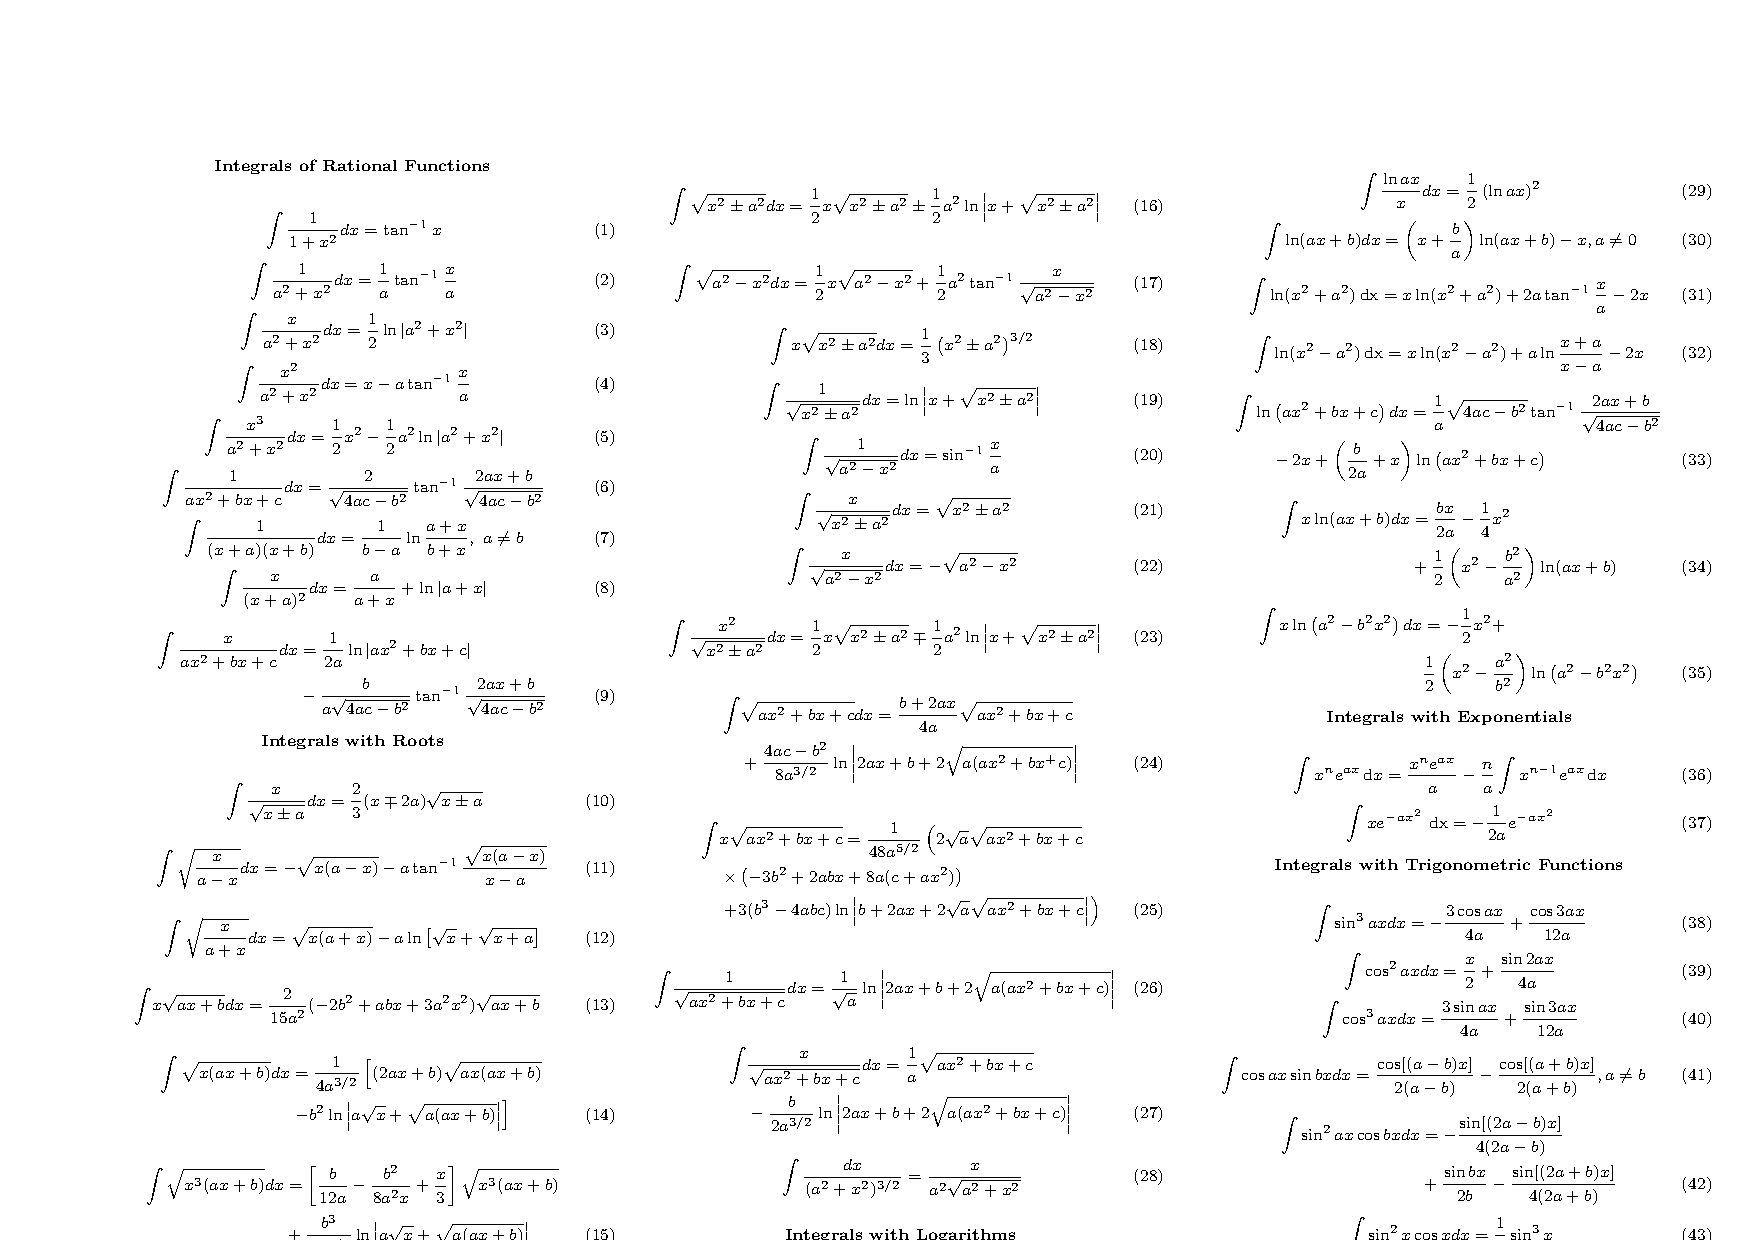
\includepdf[pages={1-2}]{./hint/Integral.pdf}

\subsection{Java}
\inputminted[breaklines]{java}{./hint/template.java}
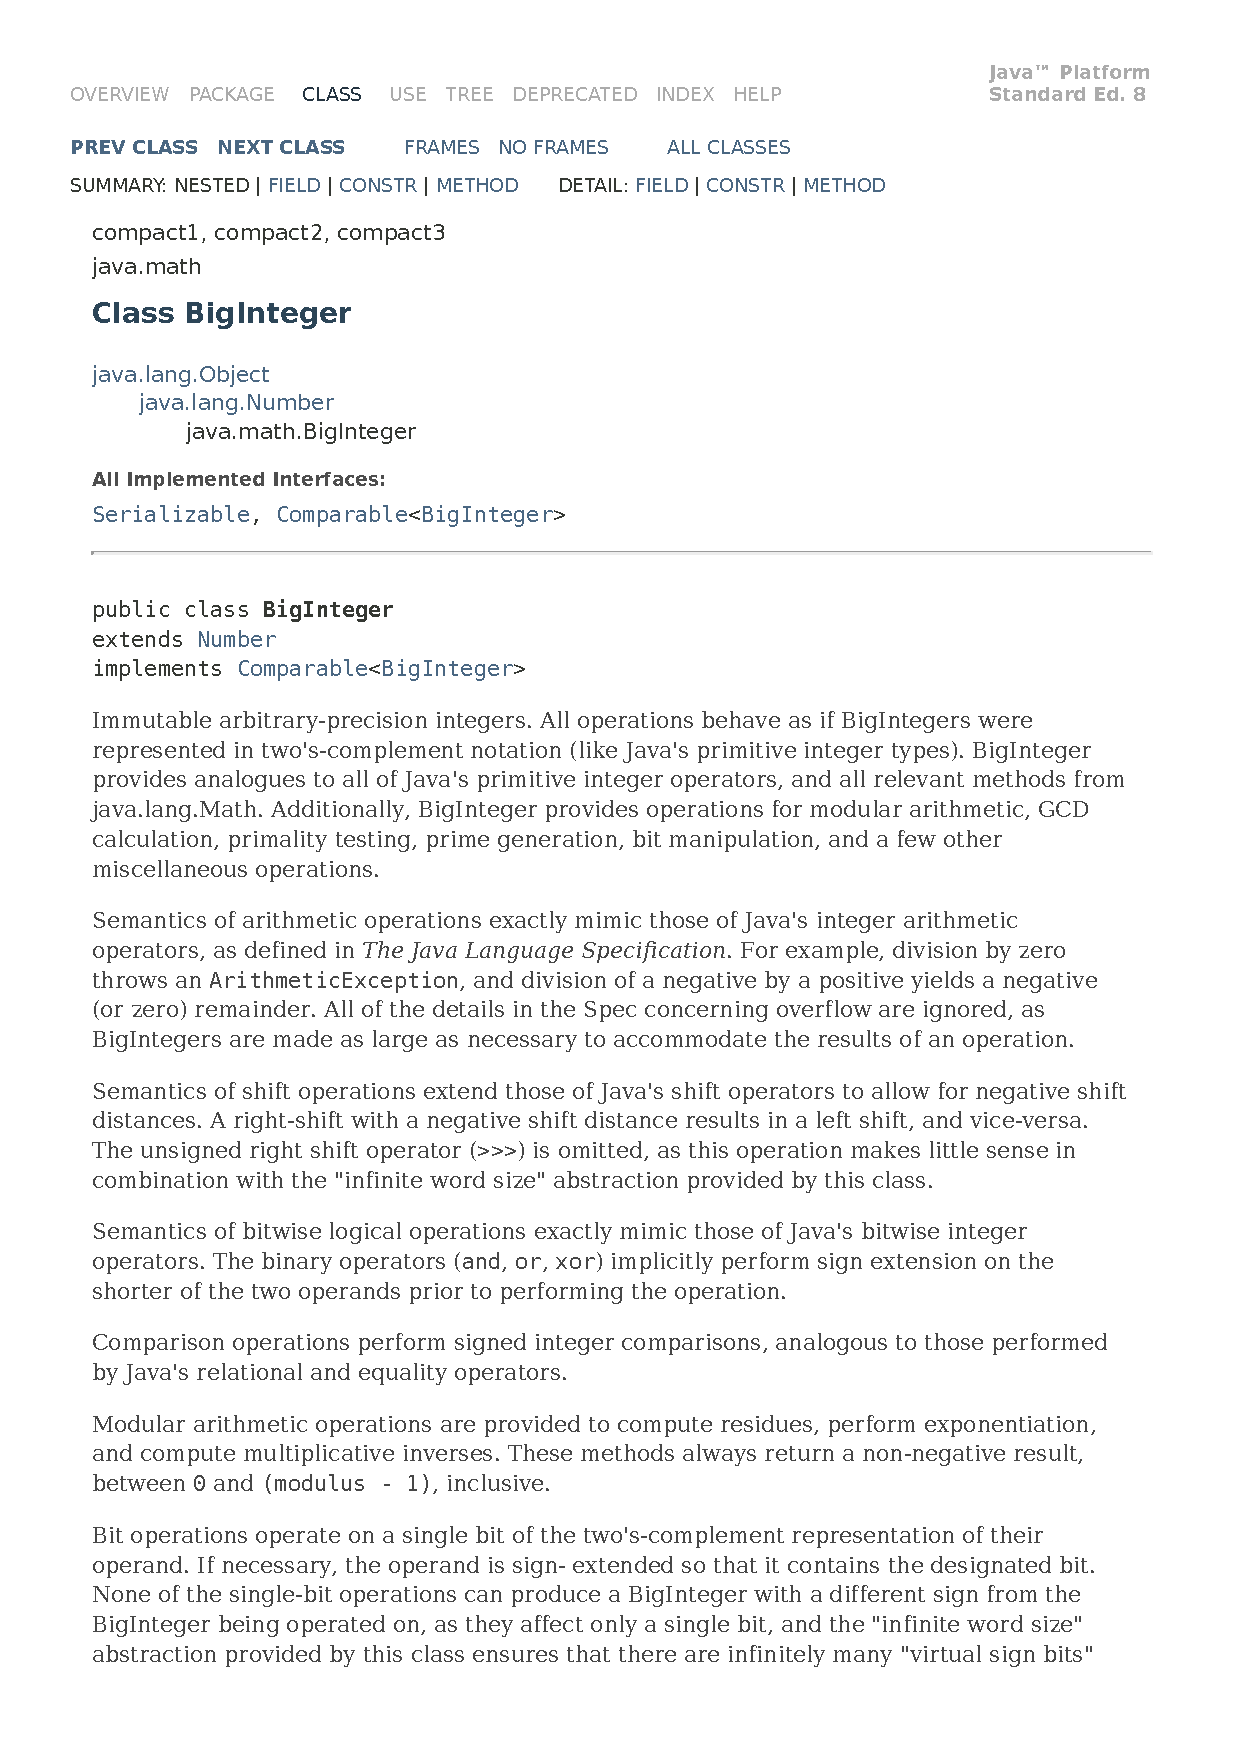
\includepdf[pages={1-6}]{./hint/biginteger.pdf}
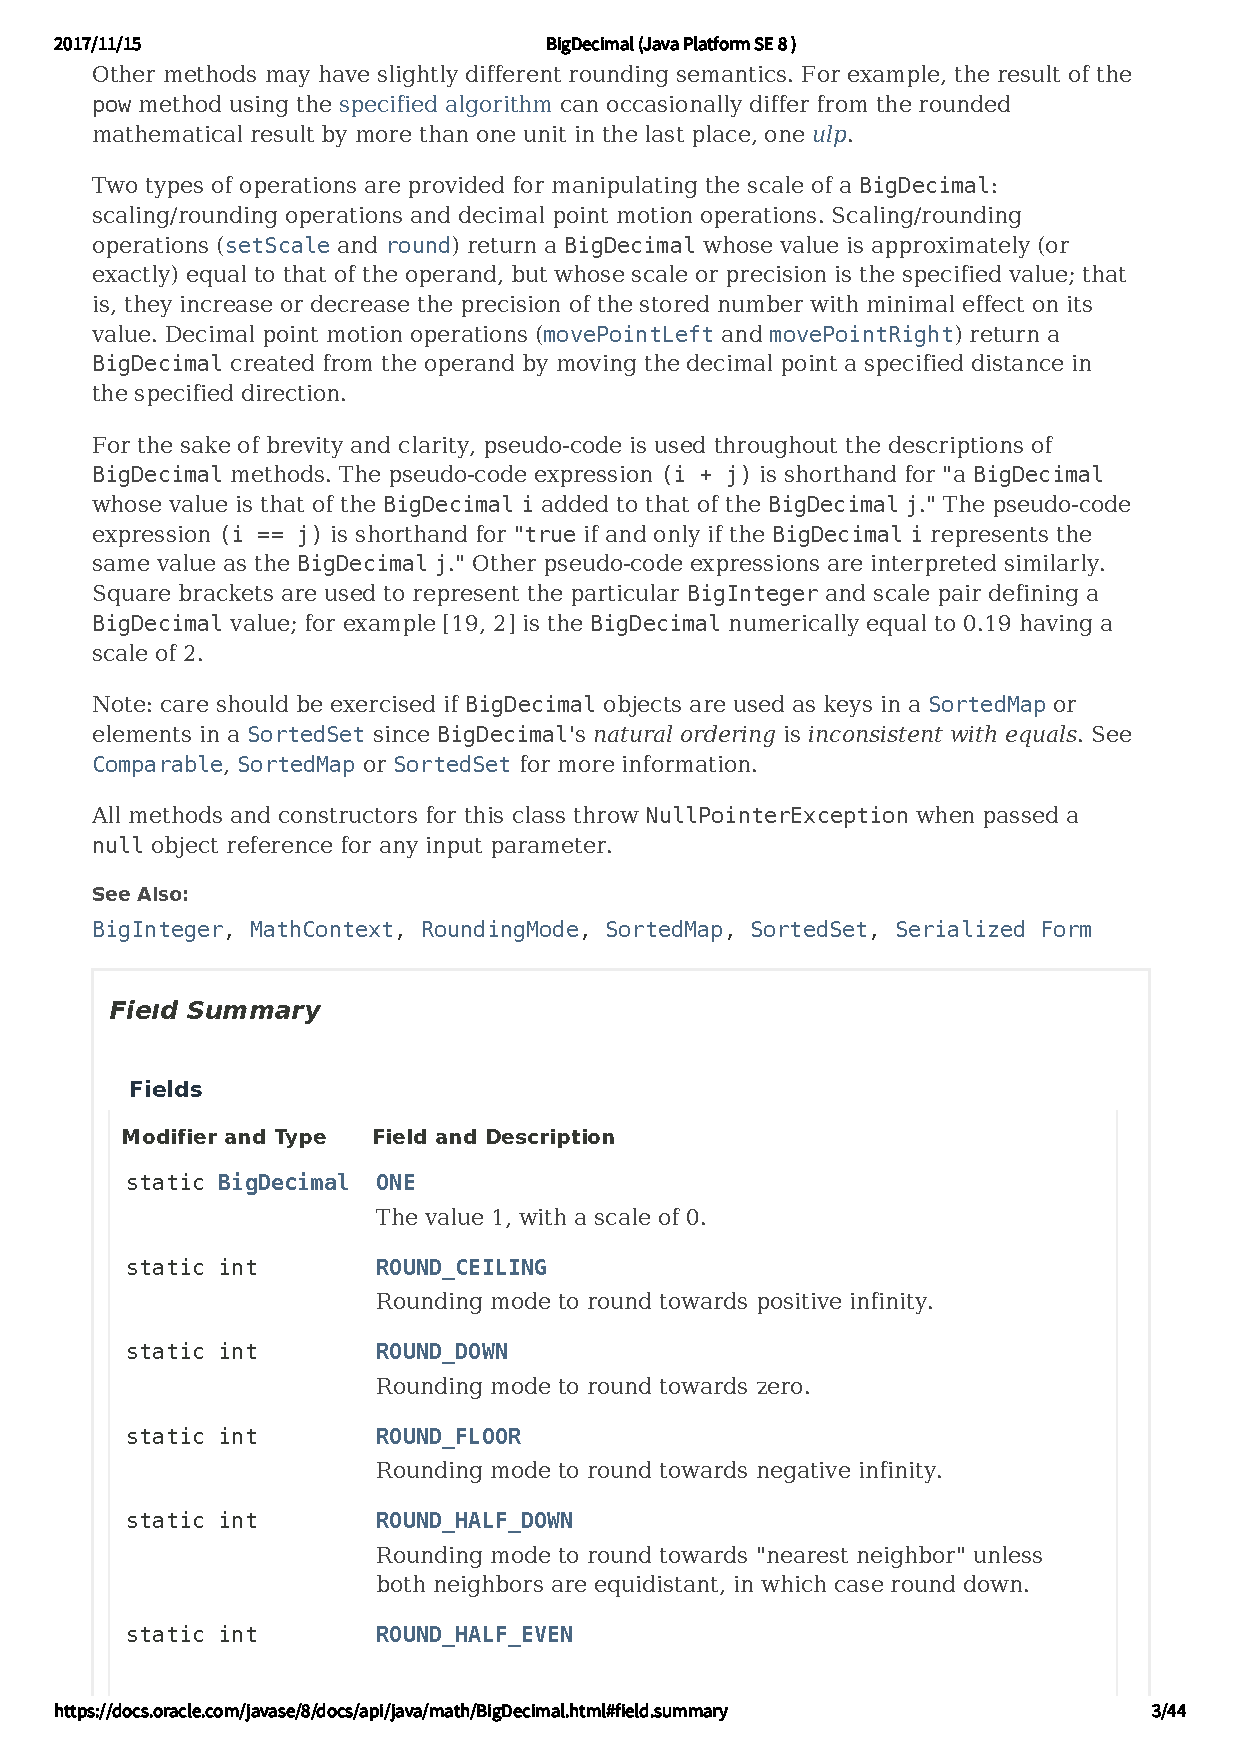
\includepdf[pages={1-7}]{./hint/BigDecimal.pdf}
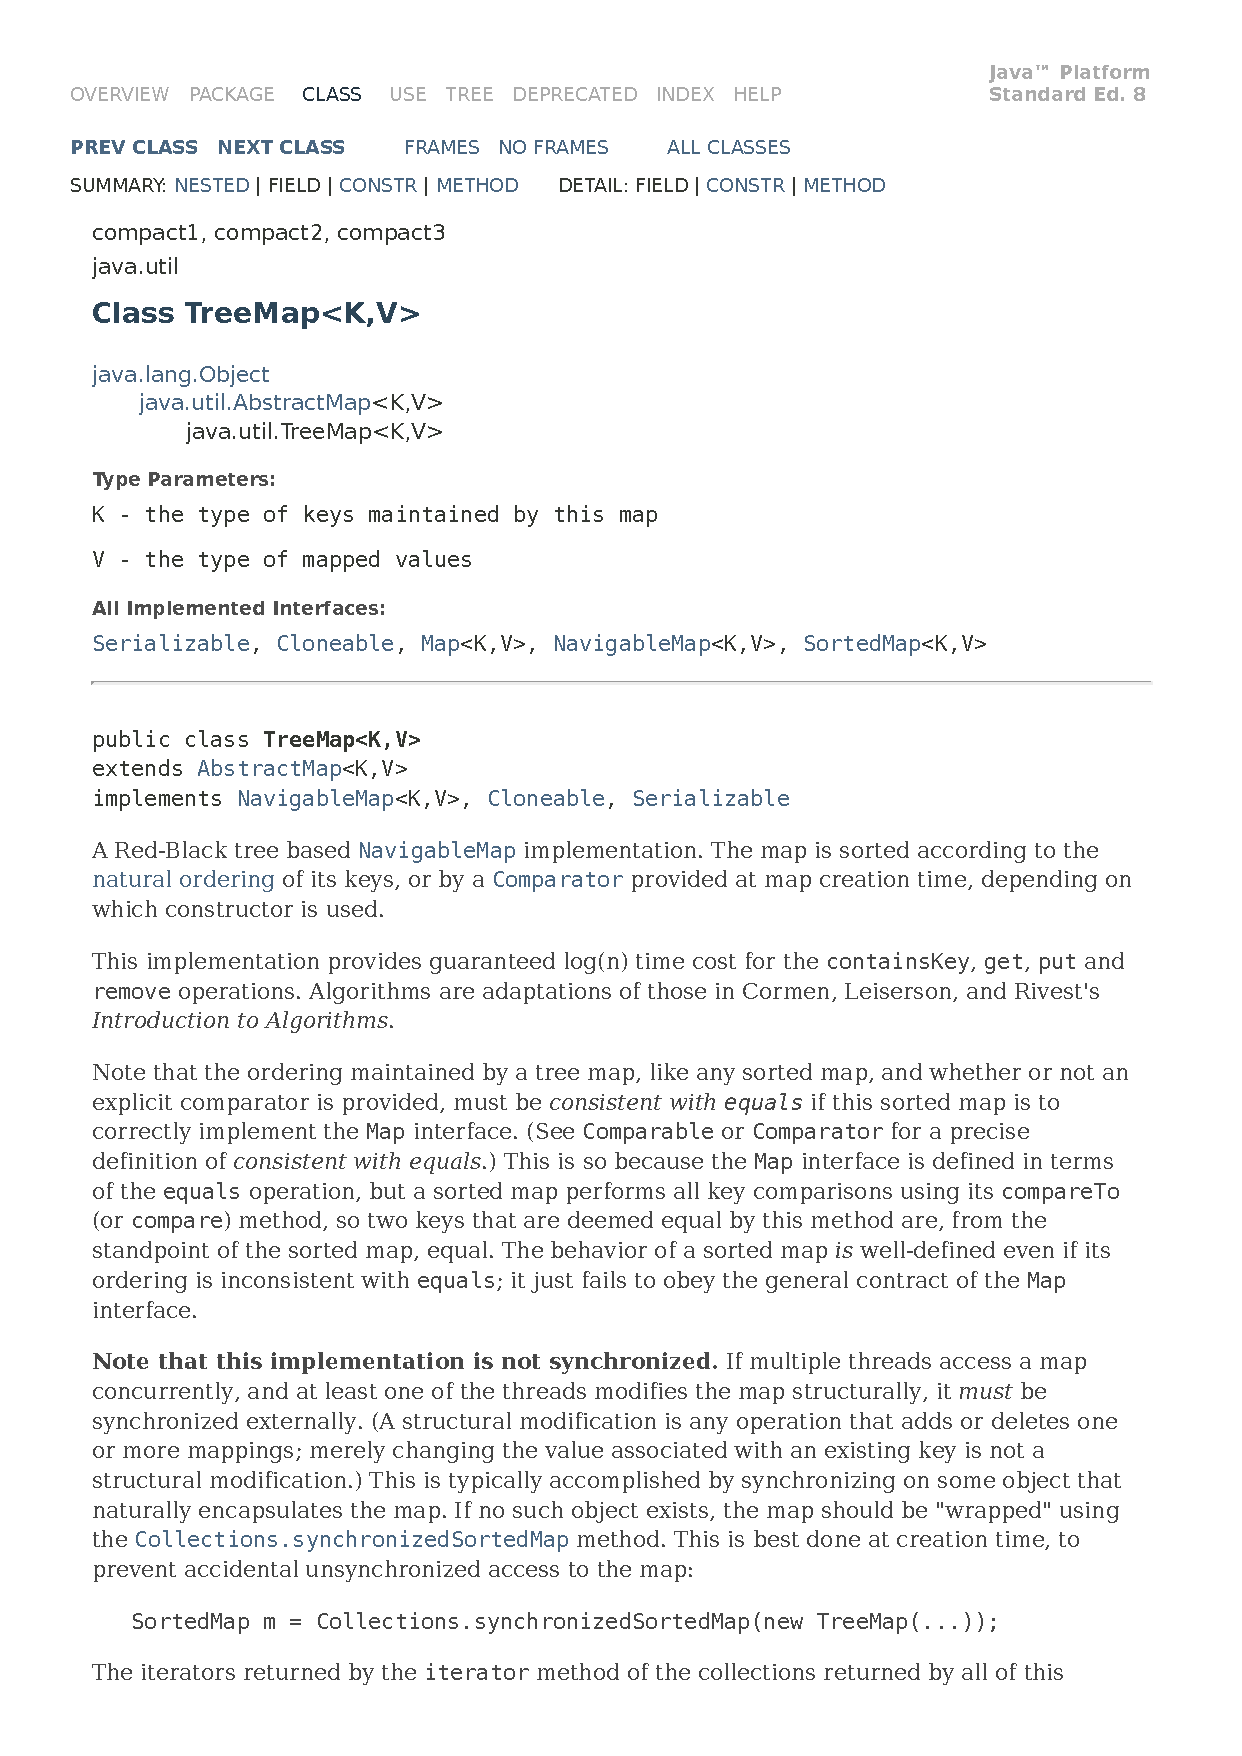
\includepdf[pages={1-5}]{./hint/treemap.pdf}
	
\end{document}
